\documentclass[a4paper,12pt]{article}
\usepackage{amsmath}
\usepackage{amssymb}
\usepackage[polish]{babel}
\usepackage{polski}
\usepackage[utf8]{inputenc}
\usepackage{indentfirst}
\usepackage{geometry}
\usepackage{array}
\usepackage[pdftex]{color,graphicx}
\usepackage{subfigure}
\usepackage{afterpage}
\usepackage{setspace}
\usepackage{color}
\usepackage{wrapfig}
\usepackage{listings}
\usepackage{datetime}

\renewcommand{\onehalfspacing}{\setstretch{1.6}}

\geometry{tmargin=2.5cm,bmargin=2.5cm,lmargin=2.5cm,rmargin=2.5cm}
\setlength{\parindent}{1cm}
\setlength{\parskip}{0mm}

\newenvironment{lista}{
\begin{itemize}
  \setlength{\itemsep}{1pt}
  \setlength{\parskip}{0pt}
  \setlength{\parsep}{0pt}
}{\end{itemize}}

\newcommand{\linia}{\rule{\linewidth}{0.4mm}}

\definecolor{lbcolor}{rgb}{0.95,0.95,0.95}
\lstset{
    backgroundcolor=\color{lbcolor},
    tabsize=4,
  language=C++,
  captionpos=b,
  tabsize=3,
  frame=lines,
  numbers=left,
  numberstyle=\tiny,
  numbersep=5pt,
  breaklines=true,
  showstringspaces=false,
  basicstyle=\footnotesize,
  identifierstyle=\color{magenta},
  keywordstyle=\color[rgb]{0,0,1},
  commentstyle=\color{Darkgreen},
  stringstyle=\color{red}
  }

\begin{document}

\noindent
\begin{tabular}{|c|p{11cm}|c|} \hline 
Grupa 6 & Wojciech Król, Maciej Kieruczenko & \ddmmyyyydate\today \tabularnewline
\hline 
\end{tabular}


\section*{Zadanie 1 - Całkowanie OpenMP}

Ćwiczenie polegało na policzeniu całki oznaczonej metodą trapezów korzystając z biblioteki OpenMP w celu zrównoleglenia obliczeń. Aby móc przekazać do programu wzór funkcji jako parametr wywołania wykorzystano bibliotekę ExprTk. Poniżej znajduje się fragment kodu, który ulega zrównolegleniu:

\begin{lstlisting}
#pragma omp parallel num_threads(nThreads) private(x,tmp) shared(from,to,nSteps)
{
	IParser* parser = parserFactory->Build();
#pragma omp for reduction(+:result)
    for (int i = 1; i < nSteps -1; i++)
    {
    	x = from + fabs(from - to) * (i / (double)nSteps);
    	tmp = parser->Eval (x);
    	result += tmp;
    }
#pragma omp single
    {
    	result += (parser->Eval (from) + parser->Eval(to)) / 2;
    }
}
return result*step;
\end{lstlisting}

Przy pomocy dyrektywy parallel przydzielono daną liczbę watków do procesu zrównoleglania. Parametr funkcji wraz z jej tymczasową wartością są prywatne dla każdego wątku, zaś przedział całkowania z liczbą trapezów są współdzielone. W celu zwiększenia wydajności przekształcono wzór liczący sumę pół trapezów umieszczając jego część w dyrektywie reduction umieszczając wartość sumy ze wszystkich wątków do jednej zmiennej globalnej oraz w dyrektywie single, która była liczona przez tylko jeden wątek.

\vspace{1cm}
Zebrano wyniki z trzech różnych funkcji oraz zestawiono poniżej w postaci dwóch wykresów - zależności przyspieszenia obliczeń oraz ich czasu od liczby wątków. Ich wzory znajdują się poniżej:

$I: f(x) = x^2 + 7x + 2$

$II: f(x) = x^3 + 4x + 13$

$III: f(x) = 4x^3 + x^2 + 8x$

\vspace{5cm}
\begin{figure}[!h]
	\centering
  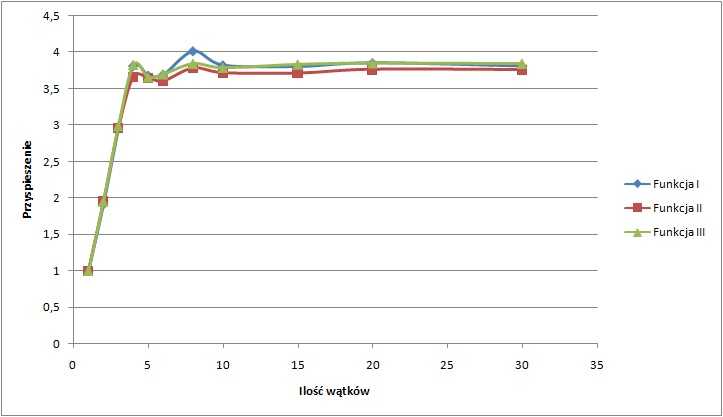
\includegraphics[width=0.6\textwidth]{wykres1.jpg}
  \caption{Wykres zależności przyspieszenia obliczeń od liczby wątków}
\end{figure}

Patrząc na powyższy wykres można zauważyć kilka zależności. Wszystkie trzy funkcje przyspieszają w niemal identyczny sposób. Przy użyciu 2-4 wątków wartość przyspieszenia była bliska idealnej, z największą zanotowaną stratą przy czterech. Lekki spadek wydajności zanotowano dla 5-7 wątków wracając do wcześniejszego stanu przy 8 i kolejnych wątkach. Zjawiska te mają miejsce z powodu narzutu tworzenia kolejnych wątków, przez co maksimum wydajności można zaobserwować dla 4 lub 8 wątków. 

\begin{figure}[!h]
	\centering
  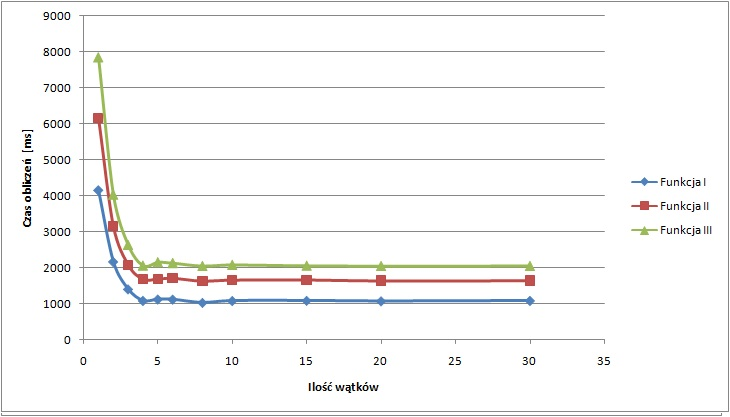
\includegraphics[width=0.6\textwidth]{wykres2.jpg}
  \caption{Wykres zależności czasu obliczeń od liczby wątków}
\end{figure}

Podobne wnioski można wysnuć obserwując drugi wykres pokazujący, jak zmienia się czas obliczeń do kolejnych wątków. Każda kolejna funkcja jest bardziej skomplikowana od poprzedniej, co wymaga więcej czasu na dokonanie obliczeń, jednakże sposób, w jaki zachowuje się wydajność jest niemal identyczny.

\vspace{1cm}
Wnioski z wykonanego ćwiczenia:
\begin{lista}
 \item Biblioteka OpenMP jest bardzo dobrym narzędziem do tworzenia programów równoległych.
 \item Otrzymane wyniki przyspieszeń są zgodne z oczekiwanymi - dla 2,3 i 4 wątków następuje wzrost wydajności, następnie występuje jej lekki spadek, po czym utrzymuje stały poziom.
 \item Poziom skomplikowania funkcji wplywa na czas jej obliczeń.
\end{lista}

\end{document}
